\id{МРНТИ 81.93.29}{}

\begin{articleheader}
\sectionwithauthors{А.С.Амирова, А.А.Құттыбек, М.М.Есмагамбетова, Т.У.Есмагамбетов }{АНЫҚ ЕМЕС ЛОГИКАҒА НЕГІЗДЕЛГЕН АҚПАРАТТЫҚ ҚАУІПСІЗДІК ҚАТЕРДІ БАҒАЛАУ МОДЕЛІ}

{\bfseries
\textsuperscript{1}А.С.Амирова\textsuperscript{\envelope } \authorid
\textsuperscript{1}А.А.Құттыбек\authorid,
\textsuperscript{1}М.М.Есмагамбетова\authorid,
\textsuperscript{1}Т.У.Есмагамбетов\authorid}
\end{articleheader}

\begin{affiliation}
\emph{\textsuperscript{1}Astana IT University, Астана, Қазақстан,}

\emph{\textsuperscript{2}Қазтұтынуодағы Қарағанды университет}

\textsuperscript{\envelope }Корреспондент-автор: akzhibek.amirova@astanait.edu.kz
\end{affiliation}

Мақалада өнеркәсіптік заттардың интернеті (IIoT- Industrial Internet of
Things) ортасындағы ақпараттық қауіпсіздік мәселесі қарастырылады. IIoT
- тегі ақпараттық қауіпсіздік қатерлерді бағалау бірқатар факторлармен
қиындайды: жүйенің күрделілігі мен біртектілігі, жүйенің динамикасы,
таратылған желілік инфрақұрылым, стандарттар мен нұсқаулықтардың
болмауы, сондай-ақ қауіпсіздіктің бұзылуының жоғарылауы. Осы сынды
факторларды ескере отырып, IIoT-те ақпараттық қауіпсіздік қатерлерін
бағалау белгілі бір жүйе мен саланың ерекшеліктері мен талаптарына
бейімделген кешенді тәсілді қажет етеді. Қатерлерді бағалаудың
мамандандырылған әдістерін қолдану және жүйенің контексті мен
ерекшеліктерін ескеру қажет. Анық емес жиындар теориясының математикалық
аппаратына негізделген IIoT-те ақпараттық қауіпсіздік қатерлерін бағалау
әдісі ұсынылған. Бұл мақалада IIoT жүйелеріне ақпараттық қауіпсіздік
қатерлеріне талдау жүргізілді, оның ішінде ең маңызды критерийлер
таңдалды. Шешімдердің негізінде қабылданатын ережелер кіріс параметрлері
бар логикалық формулалар түрінде тұжырымдалады. Үш анық емес
қорытындылар жүйесі қолданылады: біріншісі қауіптің туындау ықтималдығын
бағалау үшін, екіншісі ықтимал залалды бағалау үшін және соңғысы IIoT
жүйесі үшін ақпараттық қауіпсіздік қатерді бағалау үшін. Ұсынылған әдіс
негізінде IIoT ортасында ақпараттық қауіпсіздік қатерлерді бағалауды
есептеу мысалдары келтірілген. Ұсынылған ғылыми тәсіл IIoT жүйелерін
жобалау үшін сараптамалық шешімдерді қолдау жүйелерін құру үшін негіз
бола алады

{\bfseries Түйін сөздер:} өнеркәсіптік заттардың интернеті, тәуекелді
бағалау, лингвистикалық айнымалылар, қауіптер, анық емес логика.

\begin{articleheader}
{\bfseries МОДЕЛЬ ОЦЕНКИ РИСКОВ ИНФОРМАЦИОННОЙ БЕЗОПАСНОСТИ НА БАЗЕ НЕЧЕТКОЙ ЛОГИКИ}

{\bfseries
\textsuperscript{1}А.С.Амирова\textsuperscript{\envelope },
\textsuperscript{1}А.А.Құттыбек,
\textsuperscript{2}М.М.Есмагамбетова,
\textsuperscript{2}Т.У.Есмагамбетов}
\end{articleheader}

\begin{affiliation}
\emph{\textsuperscript{1}Astana IT University, Астана, Казахстан,}

\emph{\textsuperscript{2} Карагандинский университет Казпотребсоюза, Караганда, Казахстан,}

e-mail: akzhibek.amirova@astanait.edu.kz
\end{affiliation}

В данной статье рассматривается проблема информационной безопасности в
среде промышленного Интернета вещей (IIoT- Industrial Internet of
Things). Оценка рисков информационной безопасности в IIoT осложняется
рядом факторов: сложностью и неоднородностью системы, динамичностью
системы, распределенной сетевой инфраструктурой, отсутствием стандартов
и руководств, а также возросшими последствиями нарушений безопасности.
Учитывая эти факторы, оценка рисков информационной безопасности в IIoT
требует комплексного подхода, адаптированного к особенностям и
требованиям конкретной системы и отрасли. Необходимо использовать
специализированные методы оценки рисков и учитывать контекст и
особенности системы. Предложен метод оценки рисков информационной
безопасности в IIoT, основанный на математическом аппарате теории
нечетких множеств. В данной работе проведен анализ угроз информационной
безопасности для систем IIoT, из которого выбраны наиболее значимые
критерии. Правила, на основе которых принимаются решения, сформулированы
в виде логических формул, содержащих входные параметры. Используются три
системы нечеткого вывода: одна для оценки вероятности реализации угрозы,
другая для оценки вероятного ущерба и финальная для оценки риска
информационной безопасности для системы IIoT. На основе предложенного
метода приведены примеры расчета оценки риска информационной
безопасности в среде IIoT. Предложенный научный подход может служить
основой для создания экспертных систем поддержки принятия решений для
проектирования систем IIoT.

{\bfseries Ключевые слова:} промышленный интернет вещей, оценка риска,
лингвистические переменные, угрозы, нечеткая логика.

\begin{articleheader}
{\bfseries INFORMATION SECURITY RISK ASSESSMENT MODEL BASED ON FUZZY LOGIC}

{\bfseries
\textsuperscript{1}A.S.Amirova\textsuperscript{\envelope },
\textsuperscript{1}A.A.Kuttybek,
\textsuperscript{2}M.M. Yesmagambetova,
\textsuperscript{2}T.U. Yesmagambetov}
\end{articleheader}

\begin{affiliation}
\textsuperscript{1} Astana IT University, Астана, Kazakhstan,

\textsuperscript{2} Karaganda University of Kazpotrebsouz, Karaganda, Kazakhstan,

email: akzhibek.amirova@astanait.edu.kz
\end{affiliation}

This article discusses the problem of information security in the
Industrial Internet of Things (IIoT) environment. Assessing information
security risks in IIoT is complicated by a number of factors: system
complexity and heterogeneity, system dynamism, distributed network
infrastructure, lack of standards and guidelines, and increased
consequences of security breaches. Given these factors, assessing
information security risks in IIoT requires an integrated approach
adapted to the features and requirements of a specific system and
industry. It is necessary to use specialized risk assessment methods and
take into account the context and features of the system. A method for
assessing information security risks in IIoT based on the mathematical
apparatus of fuzzy set theory is proposed. In this paper, an analysis of
information security threats to IIoT systems is conducted, from which
the most significant criteria are selected. The rules on the basis of
which decisions are made are formulated as logical formulas containing
input parameters. Three fuzzy inference systems are used: one to assess
the probability of a threat being realized, another to assess the
probable damage, and the final one to assess the information security
risk for the IIoT system. Based on the proposed method, examples of
calculating the information security risk assessment in the IIoT
environment are given. The proposed scientific approach can serve as a
basis for creating expert decision support systems for designing IIoT
systems.

{\bfseries Keywords:} industrial internet of things, risk assessment,
linguistic variables, threats, fuzzy logic.

\begin{multicols}{2}
{\bfseries Кіріспе.} Өнеркәсіптік заттардың интернеті (IIoT- Industrial
Internet of Things) жобалау мен өндірістен бастап операцияларға, жеткізу
тізбегі мен қызмет көрсетуге дейін өнеркәсіптік операциялардың барлық
кезеңдерін автоматтандыру үшін интеллектуалды, өзара байланысты
киберфизикалық жүйелерді пайдалана отырып, тез шындыққа айналуда. IIoT
революциялық өнімділікті арттыру үшін икемді және ақылды өндірістің
күшін пайдалану арқылы өңдеуші салалардың болашағын қалыптастырады.

Саланың цифрлық құрамдас бөлігінің дамуын шектейтін ең маңызды
факторлардың бірі ақпараттық қауіпсіздіктің жеткіліксіздігі болып
табылады. Төртінші өнеркәсіптік революция және бүкіл әлем бойынша
қосылған құрылғылар санының экспоненциалды өсуі, киберқауіпсіздік
инциденттерінің санының жылдам өсуімен бірге, әсіресе Интернет заттары
шешімдерін қабылдай бастаған өнеркәсіптік операторлар арасында кибер
тұрақтылықты жақсарту қажеттілігін одан әрі көрсетеді. Индустрия 4.0
және Smart Manufacturing бойынша соңғы бастамалар технологиялық
шешімдердің қауіпсіздігіне және оларға сенетін азаматтардың
қауіпсіздігіне қатысты аспектілерге көбірек назар аударады. Бұл тақырып
одан да маңыздырақ, өйткені жаңа қауіптердің ықтимал әсері
қауіпсіздіктің физикалық бұзылуынан бастап жабдықтың зақымдалуына,
өнімнің бүлінуіне, өндірістің тоқтап қалуына және нәтижесінде қаржылық
және беделді жоғалтуларға дейін болады.

Ақпараттық қауіпсіздік жүйесін енгізудің негізгі кезеңі кәсіпорынның
жұмысы ұшырауы мүмкін тәуекелдерді бағалау болып табылады. Бұл кезең
кәсіпорында жасалып жатқан киберқауіпсіздік жүйесіндегі басымдықтарды
белгілеуге көмектеседі.

NIST SP 800-39 және ISO/IEC 27005 сияқты кәсіпорынның ақпараттық
тәуекелдерін бағалаудың бірнеше стандарттары мен әдістемелері бар. Олар
бағалаудың жалпы принциптерін түсіндіріп, кейбір нұсқауларды ұсынса да,
кибершабуыл сценарийін қалай жүзеге асыру керектігі туралы толық мәлімет
бермейді. Сонымен қатар, бұл стандарттар Өнеркәсіптік заттардың
Интернеті жүйелерінің тәуекелдерін бағалау бойынша ұсыныстар бермейді.

Сондықтан, IIoT жүйелерінің ақпараттық қауіпсіздік қатерлерді бағалаудың
практикалық үлгісін әзірлеу өзекті және зерттелетін міндет болып
табылады, оның шешімін көптеген өнеркәсіптік кәсіпорындар күтіп отыр.

{\bfseries Материалдар мен тәсілдер}. IIoT қауіпсіздігі саласындағы ең
ауқымды зерттеулердің бірі {[}1-3{]} жұмыстар болып табылады. Егер {[}1,
б. 1-9{]} жалпы Индустрия 4.0 жүйелік архитектурасына арналған және
қауіпсіздікке бағытталған архитектуралық ұсыныстардың артуын атап өтеді,
бірақ қауіпсіздікті егжей-тегжейлі талқыламайды, содан кейін {[}2, б.
4724-4733{]} бар шабуылдарды зерделеу арқылы бірінші кезекте қауіп
сипаттамасына назар аударады. Сонымен қатар, жоғарыда аталған
зерттеулерде авторлар дәстүрлі қауіпсіздік стратегиясы жеткіліксіз және
IIoT-ға дайын емес деген пікірмен келісетінін атап өткен жөн.

Авторлар {[}4{]} Microsoft STRIDE, OWASP және ENISA классификациясы
сияқты АТ-инфрақұрылымына қауіптерді анықтауға арналған модельдер заттар
интернетінің қауіптерін толық сипаттайтынына, бірақ олардың қатерлерін
толық анықтай алмайтынына назар аударылады. Осыған байланысты өндірістік
жүйелерге қауіптердің дұрыс жіктелуін анықтау мәселесі туындайды.

Мысалы, {[}5{]} IIoT бейімделетін салаларға ықтимал қауіпсіздік
қатерлерін талдады, деңгейлі IIoT архитектурасының құрамдас бөліктері
ұшырауы мүмкін шабуылдарды зерттеді және кейбір алдын алу шараларын
ұсынды. IIoT шабуылдарының таксономиясы ұсынылды, бұл авторлардың
пікірінше, шабуылдардың қаупін азайтуға көмектеседі. Бұл таксономия төрт
өлшем бойынша қарастырылды: шабуыл векторы, шабуыл нысанасы, шабуылдың
әсері және шабуылдың салдары. Дегенмен, бұл таксономияның кемшілігі
қарастырылатын қауіптердің шектеулі саны болып табылады, бұл жағдайдың
бүкіл бейнесін толығымен қамтуға мүмкіндік бермейді.

{[}6{]} мақаласында авторлар спуфинг, SQL инъекциялары, DOS шабуылдары
сияқты қауіптердің кейбір түрлерін бес деңгейлі IIoT архитектурасының
құрамдас бөліктері контекстінде қарастырды. Авторлар IIoT қатерлерін
дәлірек және толық жіктеу үшін қосымша зерттеулер қажет екенін атап
өтті.

Зерттеуге {[}7{]} назар аударған жөн, мұнда IEC 62443 стандарты
негізінде IIoT ортасында қауіпсіздік тәуекелдерін бағалау моделі
жасалған. Осы мақалада зерттелген модель анықталған осалдықтарды ескере
отырып, өнеркәсіптік қондырғы ұшырайтын тәуекелдерді барынша дәл
бағалауға арналған. Мақалада сипатталған артықшылықтарға қарамастан,
бағалау үлгісі жүйенің тұтастығы, ресурстардың қолжетімділігі сияқты
қауіпсіздік талаптарын қарастырмайды және модель IIoT жүйесіне
қауіптердің әсерін азайту шараларын ұсынбайды.

Әдебиеттерді шолу өнеркәсіптік IoT ақпараттық қауіпсіздігін қамтамасыз
ету мәселесін зерттеудің маңыздылығы мен өзектілігін растайды. Атап
айтқанда, қауіпті жіктеу, активтерді сәйкестендіру және IIoT жүйелерінің
қауіпсіздік тәуекелдерін талдау сияқты мәселелер. Сондай-ақ,
зерттеулердің талдауы зерттеулердің айтарлықтай көлемі қауіпсіздік
шараларын анықтауға арналғанын көрсетеді, ал алдын алу шаралары
мәселесі, оның ішінде ақпараттық қауіпсіздік тәуекелдерін талдау дерлік
зерттелмеген.

Бүгінгі таңда әлсіз құрылымдалған және нашар формалданған құбылыстар мен
процестерді талдау, болжау және модельдеу саласындағы ғылыми
зерттеулердің ең перспективалы құралдарының бірі американдық ғалым Лотфи
Заде алғаш рет ұсынған анық емес жиындар теориясы және анық емес логика
болып табылады {[}8{]}. Бұл теория шындықтың математикалық сипаттамасын
сөзсіз сүйемелдейтін белгісіздіктің әртүрлі формаларын есепке алу
мүмкіндіктерін айтарлықтай кеңейтеді. Осы сынды тәсіл, болып жатқан
процестер туралы толық емес және анық емес ақпарат, шектеулі және
сенімсіз білім жағдайында, сондай-ақ бағалауда субъективтілік болған
кезде әртүрлі жүйелердің жұмысын жақсарту мәселелерін шешуді қамтамасыз
етеді.

Модельдеудің әрбір кезеңінде заңдылықтарды нақты және бір мағыналы
тұжырымдауды талап ететін дәстүрлі математикадан айырмашылығы, анық емес
логика ойлаудың баламалы деңгейін ұсынады. Бұл тәсілде шығармашылық
модельдеу процесі үлгілердің ең аз жиынтығы ғана болжамданатын жоғары
деңгейде жүреді {[}9{]}.

Ақпараттық қауіпсіздік саласында бұл мәселе өте өзекті болып қала
береді. Бір жағынан шешім қабылдаудағы дәлдік пен оңтайлылық максималды
тиімділікті қамтамасыз ететін табысты қауіпсіздік стратегиясында шешуші
рөл атқарады. Екінші жағынан, ақпараттық қауіпсіздікті бағалау мен
басқаруда кездейсоқтық пен дәлсіздік факторлары бар {[}10{]}.

Ақпараттық қауіпсіздікті (АЖ) бағалауға жарамды анық емес модельді жасау
үшін анық емес жиындар теориясы негізінде бар модельдердің
мүмкіндіктерін талдау қажет.

Анық емес A ̃ жиыны реттелген жұптар жиыны ретінде түсіндіріледі
\(\left\{ \left( x_{i}|\mu_{\widetilde{A}}(x_{i}) \right) \right\}\),,
мұндағы \(\mu_{\widetilde{A}}(x_{i})\) - элементтің осы жиынға мүшелік
дәрежесін сипаттайтын x\_i элементінің мүшелік функциясы {[}11{]}.

формулаға сәйкес келесі үш жағдай мүмкін:

\begin{equation}
\begin{aligned}
    \mu_{A}(x) &= 0  \\
    0 < \mu_{A}(x) &< 1 \\
    \mu_{A}(x) &= 1
\end{aligned}
\end{equation}

Мұндағы, \(\mu_{A}(x) = 0\), егер \emph{x} элементі \emph{А} жиынына
қосылмаса,

\(0 < \mu_{A}(x) < 1\), егер \emph{x} элементі ішінара \emph{A} жиынына
қосылса,

\(\mu_{A}(x) = 1\), егер \emph{x} элементі толық \emph{A} жиынына
қосылса.

Қазіргі уақытта анық емес модельдің ең көп қолданылатын түрі - Мамдани
моделі {[}12{]}. Бұл модель шамадан тыс есептеулерді болдырмайтын анық
емес қорытындыға негізделген. Бұл алгоритм анық емес модельдеу
есептерінде кең практикалық қолдануды алды және оның «қара жәшік»
принципінде жұмыс істеуімен ерекшеленеді. Сандық мәндер кіріс ретінде
қабылданады, ал бірдей сандық мәндер шығарылады. Аралық кезеңдерде анық
емес логика және анық емес жиындар теориясының аппараты қолданылады.
Мамдани моделінің пайдасына таңдау оның жақсы лингвистикалық
түсіндірмелілігімен түсіндіріледі, бұл көбінесе оны өнеркәсіптік IoT
жүйелерінде қолданудың қарапайымдылығын анықтайды.

Мамдани моделі келесі кезеңдерден тұрады {[}13{]}:

1. Фаззификация: анық емес айнымалылар мен мүшелік функцияларды анықтау.

2. Анық емес өндіріс ережелерінің негізін қалыптастыру.

3. Анық емес өндірістер ережелеріндегі ішкі шарттарды біріктіру.

4. Анық емес өндіріс ережелерінің қорытындыларын жинақтау.

5. Шығарылатын мәннің дефаззификациясы.

Блоктардың әрқайсысын толығырақ қарастырайық.

Мамдани моделінің бірінші кезеңі анық емес айнымалылар мен мүшелік
функцияларын анықтау болып табылады. Анық емес айнымалылар жүйенің
кірістері мен шығыстарын сипаттайды және олардың мәндері мен мүшелік
функцияларымен сипатталады. Фаззификация мақсаты анық емес қорытындылар
жүйесінің жеке кіріс айнымалысының нақты, әдетте сандық мәні мен кіріс
тілдік айнымалының сәйкес терминінің мүшелік функциясының мәні
арасындағы сәйкестікті орнату болып табылады. Осы кезеңді аяқтағаннан
кейін барлық кіріс айнымалылар үшін анық емес қорытындылар жүйесінің
ережелер базасының ішкі шарттарында қолданылатын әрбір тілдік терминдер
үшін мүшелік функциялардың нақты мәндері анықталуы керек {[}14{]}.

Фаззификация кезеңі мыналарды қамтиды:

1. Кіріс және шығыс лингвистикалық айнымалылардың санын анықтаңыз.

2. Әрбір LP үшін терминдер санын орнатыңыз.

3. Әрбір ЖЖ-ның әрбір мүшесі үшін ТҚ құрыңыз.

Екінші кезең кіріс және шығыс айнымалыларды байланыстыратын анық емес
қорытындылар жүйесі ережелерінің негізін қалыптастырудан тұрады.
Ережелер лингвистикалық терминдерді және «ЖӘНЕ», «НЕМЕСЕ» және «ЕМЕС»
сияқты анық емес логикалық операторларды пайдалана отырып, қорытынды
шарттар ретінде тұжырымдалған. Әрбір ереже кіріс айнымалыларының
ағымдағы мәндеріне негізделген қандай шығысты шығару керектігін
анықтайды.

Ережелердің анық емес базасы (бұлыңғыр өнімді) зерттелетін объектінің
кірістері мен шығыстары арасындағы байланысты анықтайтын анық емес
«ЕГЕР-ОНДА» ережелерінің жиынтығы {[}15{]}.

Үшінші кезең -- ішкі шарттарды біріктіру және қорытындыларды жинақтау:
Бұлыңғыр өндірістер ережелеріндегі ішкі шарттарды жинақтау бірнеше ішкі
шарттарды бір, неғұрлым жалпы шартқа біріктіруден тұрады. Бұл ережелерді
жеңілдетуге және оларды қысқаша етуге мүмкіндік береді. Бұл қадамда
белсендірілген ережелер мен олардың шығыстары анық емес жүйенің жалпы
нәтижесін алу үшін біріктіріледі. Әрі қарай анық емес өндіріс
ережелерінің қорытындылары жинақталады. Қорытынды жинақтау дәлірек
нәтиже алу үшін анық емес ережелердің қорытындылары біріктірілгенін
білдіреді.

Соңғы кезең - дефаззификация. Шығарылатын мәнді дефаззифилау оны анық
емес мәннен нақты мәнге түрлендіруді қамтиды. Мамадани үлгісіндегі
дефаззификация әдісі ауырлық центрі әдісі болып табылады, ол шығыс
айнымалының меншікті мәнін анықтау үшін анық емес шығыстың масса центрін
есептейді {[}16{]}.

Дефаззификацияяның бірнеше әдістері бар. Бұл мақалада орташа өлшенген
максималды әдіс қолданылады. Бұл әдіс барлық қолданылатын мүшелік
функциялары максималды мәнге жететін мәндердің мүшелік бойынша өлшенген
орташа мәнін шығарады. (2) формуласы есептеу үшін пайдаланылады
{[}17{]}:

\begin{equation}
    Z = \frac{\sum_{i = 1}^{n}{\mu_{i}x_{i}}}{\sum_{i = 1}^{n}\mu_{i}}
\end{equation}

мұндағы \emph{n} -- квантталған шығыс түйреуіштердің саны;

\emph{x\textsubscript{i}} -- \emph{i-}ші мүшелік функциясының
анықтамалық мәні;

\(\mu_{i}\) -- \emph{i-}ші функцияның мүшелік дәрежесі

Ақпараттық қауіпсіздік қатер деңгейі -- ақпараттық жүйеге немесе ұйымға
қауіп төну және зақымдану ықтималдығының дәрежесі.

Қауіптің жүзеге асырылуын бағалау -- келешекте қауіптің пайда болу
ықтималдығын анықтау процесі. Қауіптердің туындау ықтималдығы ақпараттық
активтердің маңыздылығы, бағдарламалық, аппараттық қамтамасыз ету,
әкімшілік және процедуралық бақылау деңгейлерінде тиісті қауіпсіздікті
басқару құралдарының болуы, сондай-ақ қауіпсіздіктің бұрынғы бұзылулары
сияқты әртүрлі факторларға байланысты болуы мүмкін. ISO/IEC 27005:2018
"Ақпараттық технологиялар. Ақпараттық қауіпсіздік тәуекелдерін бағалау
әдістері" стандартына сәйкес туындайтын қауіптердің ықтималдығын
бағалауға арналған критерийлерге мыналар жатады: активтің құны;
қолданыстағы бақылау; алдыңғы оқиғалар {[}18-20{]}.

Зиян келтіруді бағалау -- ақпарат қауіпсіздігін бұзу нәтижесінде болуы
мүмкін қаржылық, операциялық, беделді және басқа да шығындарды анықтау
процесі. Ықтимал залал өнеркәсіптік IoT жүйесінің активтеріне қауіп
төнген кезде ұйым шегуі мүмкін барлық шығындардан тұрады. FAIR
әдістемесіне сәйкес {[}21, 22{]} ықтимал залалды бағалауға арналған
критерийлерге мыналар жатады: жабдықты ауыстыру құнына байланысты залал;
жүйенің тоқтап қалуынан зақымдану; жауап беруге байланысты шығындар;
беделіне нұқсан келтіру. Алғашқы үш критерий қаржылық тұрғыдан залалға
шоғырландырылған әсер етеді, сондықтан оларды қаржылық залал ретінде
бөлек бөлген жөн. Осылайша, келтірілген залал деңгейін бағалау үшін біз
екі критерийді таңдадық: қаржылық зиян және беделге нұқсан келтіру
(материалдық емес шығындар). Таңдалған критерийлерді ескере отырып,
өнеркәсіптік IoT жүйелеріндегі ақпараттық тәуекел деңгейін бағалау
моделі әзірленді {[}23, 24{]}. Бұл модель 1-суретте берілген. Бұл
модельде ақпараттық тәуекелді бағалау процесі үш дәйекті кезеңге
бөлінген. Бірінші кезеңде У1 қауіптердің туындау ықтималдығы бағаланады,
екінші кезеңде IIoT жүйесінің қорғалған активтеріне келтірілген залалдың
бағасы У2 есептеледі. Үшінші кезеңде ақпараттық қауіпсіздік тәуекелін
бағалау R есептеледі.
\end{multicols}

{\bfseries 1 - сурет. Анық емес қорытындылар жүйесі}

\begin{multicols}{2}
Анық емес логикаға негізделген тәуекелді бағалау алгоритмін MATLAB
жүйесінің Fuzzy Logic Toolbox пакетін пайдалану арқылы енгізу ұсынылады.

2а-суретте қауіптердің ықтималдығының активтер мен бар бақылаудың
маңыздылығына тәуелділігінің 3D визуализациясы көрсетілген. Ең төменгі
бөлігі, бұл жағдайда көк түсті, қатерлердің төмен ықтималдығын
білдіреді, бұл кәсіпорын активінің тартымдылығы төмен және қолданыстағы
бақылау деңгейі жеткілікті жоғары болған кезде мүмкін болады. Айта кету
керек, ең жоғарғы бұрыш, сары өріс қауіптердің туындау ықтималдылығын
анықтайтын аймақ болып табылады.

2б-суретте қауіптердің ықтималдығының алдыңғы қауіптерге және
активтердің тартымдылығына тәуелділігінің үш өлшемді графигі
көрсетілген. График шабуылдаушылар үшін IIoT жүйесі активтерінің
маңыздылығының төмендігі және бұрынғы сирек кездесетін қауіптер
қауіптердің туындау ықтималдығының төмендігін анықтайтынын көрсетеді.

Қауіптердің ықтималдығының алдыңғы қауіптерге және бар бақылауға
тәуелділігінің үш өлшемді графигі 2в-суретте көрсетілген. Графиктегі
сары аймақ қауіптердің жоғары ықтималдығына сәйкес келетінін көрсетеді,
алдыңғы жиі кездесетін қауіптер және бар бақылаудың жеткіліксіз деңгейі.

2г суретте келтірілген залал деңгейінің қаржылық шығындарға және беделге
нұқсан келтіруге тәуелділігінің анық емес логикасына негізделген
модельдеу арқылы алынған график көрсетілген. Графиктің ең төменгі қара
көк бөлігі төмен қаржылық және беделді шығындар кезінде орын алатын
сценарийлер келтірген залалдың ең аз деңгейін көрсетеді, ал ең жоғарғы
бұрыш, сары жолақ жоғары қаржылық және беделді шығындар.
\end{multicols}

\begin{figure}[H]
	\centering
	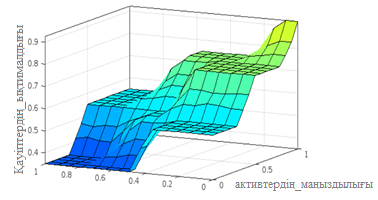
\includegraphics[width=0.8\textwidth]{media/ict/image27}
	\caption*{}
\end{figure}


а б

\begin{figure}[H]
	\centering
	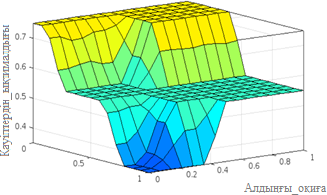
\includegraphics[width=0.8\textwidth]{media/ict/image29}
	\caption*{}
\end{figure}


в г

а - активтердің тартымдылығы және қолданыстағы бақылау туралы; б -
бұрынғы қауіптерден және активтердің тартымдылығынан; в - бұрынғы
қауіптерден және бар бақылаудан; г - келтірілген зиян деңгейінің
қаржылық шығындарға және беделге нұқсан келтіруге тәуелділігі

{\bfseries 2 - сурет. Қауіптердің ықтималдығының тәуелділігі}

\begin{multicols}{2}
{\bfseries Нәтижелер және талқылау.} Анық емес жиындар теориясы мен Мамдани
моделіне негізделген IIoT жүйелерінің ақпараттық қауіпсіздік
тәуекелдерін бағалаудың әзірленген моделі өнеркәсіптік IoT жүйелеріне
тән жоғары дәрежедегі белгісіздік жағдайында өзінің тиімділігін
көрсетті. Зерттеудің негізгі мақсаты компоненттердің өзара байланысының
жоғары дәрежесі, құрылымның күрделілігі мен қажеттілігі сияқты
өнеркәсіптік заттар интернетінің спецификалық ерекшеліктерін ескеретін
ақпараттық қауіпсіздік тәуекелдерін бағалаудың практикалық құралын жасау
болды. маңызды жүйелердің үздіксіз жұмысын қамтамасыз ету.

Осы жұмыстың нәтижелерін басқа зерттеулердің нәтижелерімен салыстыру
анық емес жиындар теориясын пайдалану әсіресе жоғары белгісіздік
жағдайында тәуекелді бағалаудың жоғары дәлдігін қамтамасыз ететінін
көрсетеді. Мысалы, ISO/IEC 27005 стандартында сипатталған тәуекелді
бағалау әдістемесі тәуекелді сапалы бағалауға ерекше мән береді, бірақ
белгісіздік жағдайында сандық талдау үшін құралдарды қамтамасыз етпейді.
Керісінше, ұсынылған модель әртүрлі кибершабуыл сценарийлерін есепке
алуға және сандық көрсеткіштерді пайдалана отырып ықтимал салдарларды
болжауға мүмкіндік береді.

Сонымен қатар, жақсы анықталған ықтималдықтарға негізделген дәстүрлі
әдістермен салыстырғанда (мысалы, NIST SP 800-39) әзірленген модель
толық емес немесе нақты емес ақпаратты қамтитын деректерді өңдеуде үлкен
икемділікті қамтамасыз етеді. Бұл деректер әртүрлі көздерден, соның
ішінде сенсорлардан, контроллерлерден және бұлттық платформалардан
алынатын, қателер мен белгісіздік ықтималдығын арттыратын IIoT жүйелері
үшін өте маңызды.

{\bfseries Қорытынды}. Мақала өнеркәсіптік IoT жүйелеріндегі ақпараттық
қауіпсіздік қатерлерді талдау мәселесін шешуге арналған. Бұл мәселені
шешу үшін анық емес логикалық әдістер қолданылды, өйткені дәл осы тәсіл
ақпаратта маңызды болып табылатын бағалаудың субъективтілігі болған
жағдайда, толық емес және дәл емес ақпарат жағдайында әртүрлі жүйелердің
жұмысын жақсарту мәселелерін шешуге мүмкіндік береді. қауіпсіздік.

Ұсынылған модель ақпараттық қауіпсіздік тәуекелдерін бағалау үшін
пайдаланылуы мүмкін, оны киберқауіпсіздік мамандары орындауы керек. Бұл
тәуекелдерді болжау және басымдық беру үшін пайдалы болуы мүмкін.
Сонымен қатар, ол тәуекелдерді бақылау және жүйелердің ақпараттық
қауіпсіздігін жақсарту бойынша шараларды жүзеге асыру саласындағы
маңызды ақпаратты ұсынады.
\end{multicols}

\begin{center}
{\bfseries Әдебиеттер}
\end{center}

\begin{references}
1. Hofer F. Architecture, technologies and challenges for cyber-physical
systems in industry 4.0: A systematic mapping study // 12th ACM/IEEE
internat. symp. Empirical Softw. Eng. Meas. -- NY., 2018. -- P. 1-10.
\href{https://doi.org/10.1145/3239235.3239242}{DOI
10.1145/3239235.3239242}

2. Sisinni E., Saifullah A., Han S. Industrial Internet of Things:
Challenges, opportunities, and directions // IEEE Trans. Ind. Informat.-
2018.-Vol.14(1) - P.4724-4734.

DOI
\href{https://doi.org/10.1109/TII.2018.2852491}{10.1109/TII.2018.2852491}

3. Tange K., De Donno M., Fafoutis X. et al. Systematic Survey of
Industrial Internet of Things Security: Requirements and Fog Computing
Opportunities // IEEE Communications Surveys \& Tutorials.- 2020.- Vol.
22(1). - P.2489-2520. DOI
\href{http://dx.doi.org/10.1109/COMST.2020.3011208}{10.1109/COMST.2020.3011208}

4. Yu X., Guo H. A Survey on IIoT Security // Procced. IEEE VTS Asia
Pacific Wireless Communications sympos//Singaporeю- 2019. -P.1-5 DOI
10.1109/VTS-APWCS.2019.8851679

5. Panchal A., Khadse V., Mahalle P. Security Issues in IIoT: A
Comprehensive Survey of Attacks on IIoT and Its Countermeasures //
Procced. 2018 IEEE Global conf. on Wireless Computing and Networking
(GCWCN).- Lonavala.- 2018.-P.124-130 DOI 10.1109/GCWCN.2018.8668630

6. Shah Y., Sengupta S. A survey on Classification of Cyber-attacks on
IoT and IIoT devices // Procced. 2020 11th IEEE Annual Ubiquitous
Computing, Electronics \& Mobile Communication conf. (UEMCON).- NY.-
2020. - P. 406-413.DOI 10.1109/UEMCON5185.2020.9298138

7. Hassani H. Vulnerability and security risk assessment in a IIoT
environment in compliance with standard IEC 62443 // Procedia Comput.
Sci.-2021.-№191.-Р. 33-40.

DOI 10.1016/j.procs.2021.07.008

8. Saaty T. What is the Analytic Hierarchy Process? // Mathematical
Models for Decision Support. -1988.-Vol.48. - P. 109-121. DOI
10.1007/978-3-642-83555-1\_5

9. Курейчик В.М. Особенности построения систем поддержки принятия
решений // Известия ЮФУ. Технические науки.- 2012. -№7(132). - С. 92-98.

10. Ani U., Tiwari A. Review of cybersecurity issues in industrial
critical infrastructure: manufacturing in perspective // Journal of
Cyber Security Technology.-2017.-Vol.1(1).- P. 32-74. DOI
10.1080/23742917.2016.1252211

11. Новак В., Перфильева И.Г., Мочкорж И. Математические принципы
нечеткой логики. -- М.: Физматлит, 2006. - 352 с. ISBN: 5-9221-0399-7

12. Абалдова С.Ю., Волынский В.Ю. Разработка системы нечеткого вывода
оценки результативности системы менеджмента качества предприятия на
основе алгоритма Мамдани // Известия высших учебных заведений. Серия:
Экономика, финансы и управление производством.- 2011. - №1.- С.86-93.

13. Голосовский М.С., Богомолов А.В., Теребов Д.С. и др. Алгоритм
настройки системы нечёткого логического вывода типа Мамдани // Вестник
Южно-Уральского государственного университета. - 2018. - № 3. - С.
19-29. DOI 10.14529/mmph180303

14. Горбачев С.В. Фаззификация экспертных лингвистических данных,
заданных в порядковой шкале // Матер. докл. 4-й междунар. заочн.
Науч.-практ. конф. «Интеллектуальные информационные системы: тенденции,
проблемы, перспективы (ИИС-2016). - Курск, 2017.- С. 47-49.

15. Belarbi K. Design of Mamdani fuzzy logic controllers with rule base
minimisation using genetic algorithm // Engineering applications of
artificial intelligence. - 2005.-Vol.18(7). - P. 875-880. DOI
10.1016/j.engappai.2005.03.003

16. Амирова А.С., Тохметов А.Т., Жанасбаева А.С. Основные проблемы
безопасности в промышленном интернете вещей // Вестник
Восточно-Казахстанского технического университета им. Д.Серикбаева. -
2021.- №1(91). -С. 82-91.

DOI 10.51885/1561-4212\_2021\_1\_82

17. Грибин М.А. Применение алгоритма Мамдани в системах автоматического
управления // Развитие современной науки: теоретические и прикладные
аспекты. -2019.- № 22. - С. 16-19.

18. ISO/IEC 27001:2022. Информационная безопасность, кибербезопасность и
защита персональных данных. URL:
https://pqm-online.com/assets/files/pubs/translations/std/iso-mek-27001-2022.pdf.
Дата обращения: 14.12.2024.

19. ISO/IEC 27005:2022. Information security, cybersecurity and privacy
protection. URL: https://www.iso.org/standard/80585. Date of address:
14.12.2024.

20. NIST SP 800-39. Managing Information Security Risk. URL:
https://nvlpubs.nist.gov/nistpubs/Legacy/SP/nistspecialpublication. Date
of address: 14.12.2024.

21. Методология FAIR (Factor Analysis of Information Risk). URL:
\url{https://www.risklens.com/hubfs/u}
ploads/2019/04/An\_Adoption\_Guide. Date of address:

14.12.2022.

22. Методология OCTAVE для оценки информационных рисков. URL:
http://www.risk24.ru/octave.htm. Дата обращения:14.12.2022.

23. Amirova A., Tokhmetov A. A model for risk analysis in the industrial
internet of things // Journal of Theoretical and Applied Information
Technology. -2021.- Vol.99(14). - P. 3449-3459.

24. Kerimkhulle S., Dildebayeva Zh., Tokhmetov А., Amirova А., Tussupov
J., Makhazhanova U., Adalbek А., Taberkhan R., Zakirova А., Salykbayeva
А. Fuzzy Logic and Its Application in the Assessment of Information
Security Risk of Industrial Internet of Things // Symmetry. -- 2023.
--Vol.15(10) - Р. 1-29. DOI10.3390/sym15101958
\end{references}

\begin{center}
{\bfseries References}
\end{center}

\begin{references}
1. Hofer F. Architecture, technologies and challenges for cyber-physical
systems in industry 4.0: A systematic mapping study // 12th ACM/IEEE
internat. symp. Empirical Softw. Eng. Meas. -- NY., 2018. -- P. 1-10.
\href{https://doi.org/10.1145/3239235.3239242}{DOI
10.1145/3239235.3239242}

2. Sisinni E., Saifullah A., Han S. Industrial Internet of Things:
Challenges, opportunities, and directions // IEEE Trans. Ind. Informat.-
2018.-Vol.14(1) - P.4724-4734.

DOI
\href{https://doi.org/10.1109/TII.2018.2852491}{10.1109/TII.2018.2852491}

3. Tange K., De Donno M., Fafoutis X. et al. Systematic Survey of
Industrial Internet of Things Security: Requirements and Fog Computing
Opportunities // IEEE Communications Surveys \& Tutorials.- 2020.- Vol.
22(1). - P.2489-2520. DOI
\href{http://dx.doi.org/10.1109/COMST.2020.3011208}{10.1109/COMST.2020.3011208}

4. Yu X., Guo H. A Survey on IIoT Security // Procced. IEEE VTS Asia
Pacific Wireless Communications sympos//Singaporeю- 2019. -P.1-5 DOI
10.1109/VTS-APWCS.2019.8851679

5. Panchal A., Khadse V., Mahalle P. Security Issues in IIoT: A
Comprehensive Survey of Attacks on IIoT and Its Countermeasures //
Procced. 2018 IEEE Global conf. on Wireless Computing and Networking
(GCWCN).- Lonavala.- 2018.-P.124-130 DOI 10.1109/GCWCN.2018.8668630

6. Shah Y., Sengupta S. A survey on Classification of Cyber-attacks on
IoT and IIoT devices // Procced. 2020 11th IEEE Annual Ubiquitous
Computing, Electronics \& Mobile Communication conf. (UEMCON).- NY.-
2020. - P. 406-413.DOI 10.1109/UEMCON5185.2020.9298138

7. Hassani H. Vulnerability and security risk assessment in a IIoT
environment in compliance with standard IEC 62443 // Procedia Comput.
Sci.-2021.-№191.-Р. 33-40.

DOI 10.1016/j.procs.2021.07.008

8. Saaty T. What is the Analytic Hierarchy Process? // Mathematical
Models for Decision Support. -1988.-Vol.48. - P. 109-121. DOI
10.1007/978-3-642-83555-1\_5

9. Kurejchik V.M. Osobennosti postroenija sistem podderzhki prinjatija
reshenij // Izvestija JuFU. Tehnicheskie nauki.- 2012. -№7(132). - S.
92-98.{[}in Russian{]}

10. Ani U., Tiwari A. Review of cybersecurity issues in industrial
critical infrastructure: manufacturing in perspective // Journal of
Cyber Security Technology.-2017.-Vol.1(1).- P. 32-74. DOI
10.1080/23742917.2016.1252211

11. Novak V., Perfil' eva I.G., Mochkorzh I.
Matematicheskie principy nechetkoj logiki. -- M.: Fizmatlit, 2006. - 352
s. ISBN: 5-9221-0399-7.{[}in Russian{]}

12. Abaldova S.Ju., Volynskij V.Ju. Razrabotka sistemy nechetkogo vyvoda
ocenki rezul' tativnosti sistemy menedzhmenta kachestva
predprijatija na osnove algoritma Mamdani // Izvestija vysshih uchebnyh
zavedenij. Serija: Jekonomika, finansy i upravlenie proizvodstvom.-
2011. - №1.- S.86-93. {[}in Russian{]}

13. Golosovskij M.S., Bogomolov A.V., Terebov D.S. i dr. Algoritm
nastrojki sistemy nechjotkogo logicheskogo vyvoda tipa Mamdani //
Vestnik Juzhno-Ural' skogo gosudarstvennogo universiteta.
- 2018. - № 3. - S. 19-29. DOI 10.14529/mmph180303.{[}in Russian{]}

14. Gorbachev S.V. Fazzifikacija jekspertnyh lingvisticheskih dannyh,
zadannyh v porjadkovoj shkale // Mater. dokl. 4-j mezhdunar. zaochn.
Nauch.-prakt. konf. «Intellektual' nye informacionnye
sistemy: tendencii, problemy, perspektivy (IIS-2016). - Kursk, 2017.- S.
47-49. {[}in Russian{]}

15. Belarbi K. Design of Mamdani fuzzy logic controllers with rule base
minimisation using genetic algorithm // Engineering applications of
artificial intelligence. - 2005.-Vol.18(7). - P. 875-880. DOI
10.1016/j.engappai.2005.03.003

16. Amirova A.S., Tohmetov A.T., Zhanasbaeva A.S. Osnovnye problemy
bezopasnosti v promyshlennom internete veshhej // Vestnik
Vostochno-Kazahstanskogo tehnicheskogo universiteta im. D.Serikbaeva. -
2021.- №1(91). -S. 82-91. {[}in Russian{]}

DOI 10.51885/1561-4212\_2021\_1\_82

17. Gribin M.A. Primenenie algoritma Mamdani v sistemah avtomaticheskogo
upravlenija // Razvitie sovremennoj nauki: teoreticheskie i prikladnye
aspekty. -2019.- № 22. - S. 16-19. {[}in Russian{]}

18. ISO/IEC 27001:2022. Informacionnaja bezopasnost',
kiberbezopasnost'{} i zashhita
personal' nyh dannyh. URL:
https://pqm-online.com/assets/files/pubs/translations/std/iso-mek-27001-2022.pdf.
Data obrashhenija: 14.12.2024. {[}in Russian{]}

19. ISO/IEC 27005:2022. Information security, cybersecurity and privacy
protection. URL: https://www.iso.org/standard/80585. Date of address:
14.12.2024.

20. NIST SP 800-39. Managing Information Security Risk. URL:
https://nvlpubs.nist.gov/nistpubs/Legacy/SP/nistspecialpublication. Date
of address: 14.12.2024.

21. Metodologija FAIR (Factor Analysis of Information Risk). URL:
\url{https://www.risklens.com/hubfs/u}
ploads/2019/04/An\_Adoption\_Guide. Date of address:

14.12.2022. {[}in Russian{]}

22. Metodologija OCTAVE dlja ocenki informacionnyh riskov. URL:
http://www.risk24.ru/octave.htm. Data obrashhenija:14.12.2022. {[}in
Russian{]}

23. Amirova A., Tokhmetov A. A model for risk analysis in the industrial
internet of things // Journal of Theoretical and Applied Information
Technology. -2021.- Vol.99(14). - P. 3449-3459.

24. Kerimkhulle S., Dildebayeva Zh., Tokhmetov А., Amirova А., Tussupov
J., Makhazhanova U., Adalbek А., Taberkhan R., Zakirova А., Salykbayeva
А. Fuzzy Logic and Its Application in the Assessment of Information
Security Risk of Industrial Internet of Things // Symmetry. -- 2023.
--Vol.15(10) - Р. 1-29. DOI10.3390/sym15101958
\end{references}

\begin{authorinfo}
\emph{{\bfseries Сведения об авторах}}

Амирова А.С. - PhD, ассистент профессор, Astana IT University, Астана,
Казахстан, e-mail:
\href{mailto:akzhibek.amirova@astanait.edu.kz}{\nolinkurl{akzhibek.amirova@astanait.edu.kz}};

Құттыбек А.А. -- сеньор-лектор, Astana IT University, Астана, Казахстан,
e-mail:
\href{mailto:azhar.kuttybek@astanait.edu.kz}{\nolinkurl{azhar.kuttybek@astanait.edu.kz}};

Есмагамбетова М.М.- PhD, доцент - Карагандинский университет
Казпотребсоюза, Караганда, Казахстан e-mail:
\href{mailto:marzhan1983@mail.ru}{\nolinkurl{marzhan1983@mail.ru}};

Есмагамбетов Т.У.- магистр, старший преподаватель - Карагандинский
университет Казпотребсоюза, Караганда, Казахстан e-mail:
\href{mailto:Timur198300@mail.ru}{\nolinkurl{Timur198300@mail.ru}}

\emph{{\bfseries Information about the authors}}

Amirova A.S. - PhD, assistant professor, Astana IT University, Astana,
Kazakhstan, e-mail:
\href{mailto:akzhibek.amirova@astanait.edu.kz}{\nolinkurl{akzhibek.amirova@astanait.edu.kz}};

Kuttybek A.A. -- senior lecturer, Astana IT University, Astana,
Kazakhstan, e-mail:
\href{mailto:azhar.kuttybek@astanait.edu.kz}{\nolinkurl{azhar.kuttybek@astanait.edu.kz}};

Yesmagambetova M.M.- PhD, assistant professor, Karaganda University of
Kazpotrebsoyuz, Karaganda, Kazakhstan e-mail:
\href{mailto:marzhan1983@mail.ru}{\nolinkurl{marzhan1983@mail.ru}};

Yesmagambetov T.U.- master, senior lecturer, Karaganda University of
Kazpotrebsoyuz, Karaganda, Kazakhstan e-mail:
\href{mailto:Timur198300@mail.ru}{\nolinkurl{Timur198300@mail.ru}};
\end{authorinfo}
